\addtolength{\oddsidemargin}{-.900in}\addtolength{\evensidemargin}{-.900in}
\addtolength{\textwidth}{1.75in}
\addtolength{\topmargin}{-.875in}
\addtolength{\textheight}{2in}
\documentclass[12pt]{homework}

\newcommand{\hwname}{Ornella Elena Grassi}
\newcommand{\hwemail}{s290310@studenti.polito.it}
\newcommand{\hwtype}{Homework}
\newcommand{\hwnum}{2}
\newcommand{\hwclass}{}
\newcommand{\hwlecture}{}
\newcommand{\hwsection}{}

% This is just used to generate filler content. You don't need it in an actual
% homework!
\usepackage{lipsum}
\usepackage{amssymb}
\usepackage[utf8]{inputenc}
\usepackage[T1]{fontenc}
\usepackage{lmodern}
\usepackage{amsfonts}
\usepackage{hyperref}
\usepackage{bbm}
\usepackage{amsmath}
\usepackage{mcode}
\usepackage{epstopdf}
\usepackage{subcaption}
\usepackage[italian]{babel}
\usepackage{ stmaryrd }

\begin{document}
\maketitle
\begin{center}
Realizzato in collaborazione con Giulio Nenna (s245717), Andrea Sanna (s222975) e Alfredo Baione (s279328)
\end{center}
\section{}% --------------ESERCIZIO 1------------------------------
  
    
    
  \begin{enumerate}
 
  
    \item[(1)]
    Dato che sono apparsi $8$ fiori tra le $9$ e le $10$ a. m.,
    \begin{itemize}
    \item
    la probabilità che $3$ di questi siano apparsi tra le $9$ e le $9:20$ a. m. è
    \begin{equation*}
    P\left(N\left(\frac{1}{3}\right)=3\mid N\left(1\right)=8\right)=\binom{8}{3}\left(\frac{1}{3}\right)^{3}\left(1-\frac{1}{3}\right)^{5}\thicksim 0.273;
    \end{equation*}
    \item
    la probabilità che ne appaiano $13$ tra le $9$ a. m. e le 11 a. m. é
     \begin{align*}
     &P\left(N\left(2\right)=13\mid N\left(1\right)=8\right)=\text{(per l'assenza di memoria)}\\
     &P\left(N\left(1\right)=5\right)=e^{-3}\frac{3^{5}}{5!}\thicksim 0.101.
     \end{align*}
    \end{itemize} 
    \item[(2)]
    Si vuole calcolare la probabilità che tra le $9$ a. m. e le $11$ a. m. compaiano esattamente $3$ fiori di tipo A, $2$ di tipo B e nessuno di tipo C.\\
    Indicando con $N_{i}\left(t\right)$ il numero dei fiori sbocciati di tipo $i$, si ottiene:
    \begin{align*}
    &P\left(N_{A}\left(2\right)=3, N_{B}\left(2\right)=2,N_{C}\left(2\right)=0\right)=\\
    &e^{-3\frac{1}{3}2}\frac{\left(3\frac{1}{3}2\right)^{3}}{3!}\cdot e^{-3\frac{1}{6}2}\frac{\left(3\frac{1}{6}2\right)^{2}}{2!}\cdot e^{-3\frac{1}{2}2}\frac{\left(3\frac{1}{2}2\right)^{0}}{0!}= \\
    &e^{-2}\frac{8}{3!}\cdot e^{-1}\frac{1}{2!}\cdot e^{-3}\thicksim 0.0016  
  \end{align*} 
  (come conseguenza del fatto che $N_{i}\left(t\right), i=A, B, C,$ sono processi di Poisson indipendenti, di rate $\lambda_{p_{i}}$).
     \item[(3)]
     Indicando con $\tau_{1}$ il tempo in cui compare il primo fiore di tipo A, risulta che se $N_{A}\left(t\right)\backsim \text{Poisson}\left(\lambda_{p_{A}}=1\right)$, allora $\tau_{1}\backsim \text{exp}\left(1\right)$.\\
     Pertanto, condizionatamente al fatto che il primo fiore che compare è di tipo A, la probabilità che il tempo $\tau$ in cui ciò avviene sia $\leq \frac{1}{2}$ è
     \begin{equation*}
     P\left(\tau_{1}\leq \frac{1}{2}\right)=\int_{0}^{\frac{1}{2}}1\cdot e^{-1\cdot x} \,dx =1-e^{-\frac{1}{2}}\thicksim 0.393.
     \end{equation*}
     
  
    

  \end{enumerate}

  \newpage
\section{}%---------------ESERCIZIO 2 2-----------------------------------
\begin{alphaparts}
    \questionpart
 Il processo di costruzione e distruzione del castello di sabbia può essere modellato con una catena di Markov a tempo continuo siffatta:                                                                        
 
\begin{figure}[htb]\centering
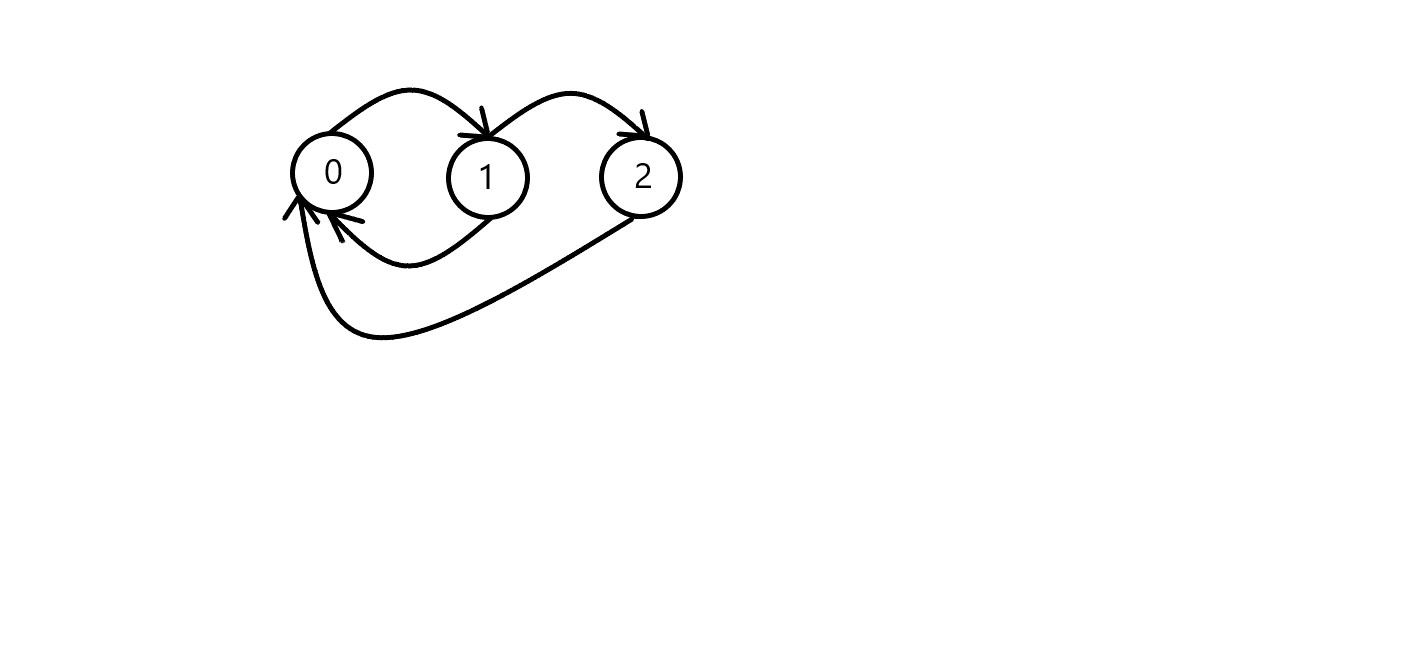
\includegraphics[scale=0.50]{catenaex2}
  \end{figure}
  
$S=\{0,1,2\}$ è l'insieme degli stati associati ai seguenti rates di permanenza in ognuno di essi:
  \begin{align*}
  &\lambda\left(0\right)=2,\\
  &\lambda\left(1\right)=\left(\frac{1}{1+3}\right)=\frac{1}{4},\\
  &\lambda\left(2\right)=3.
  \end{align*}
 La matrice di transizione della catena a tempo discreto, ovvero la catena ``embedded'', associata a tale processo, è:
 \begin{equation*}
  R=\begin{bmatrix}
        0 & 1 & 0\\
        1-e^{-3} & 0 & e^{-3} \\
         1 & 0 & 0
      \end{bmatrix}.
\end{equation*}  
Da essa è possibile ricavare la seguente matrice dei tassi di transizione $q\left(i,j\right)$($=\lambda\left(i\right)r\left(i,j\right),\forall i,j, i\neq j$):
\begin{equation*}
  Q=\begin{bmatrix}
        -2 & 2 & 0\\
        \frac{1-e^{-3}}{4} & -\frac{1}{4} &  \frac{1+e^{-3}}{4}\\
         3 & 0 & -3
      \end{bmatrix}.
\end{equation*}  
\questionpart
La probabilità che, partendo dallo stato $1$, dopo $2$ ore, ci si ritrovi nello stato $0$ è
\begin{equation*}
P_{2}\left(1,0\right),
\end{equation*} 
dove $P_{2}$ è la matrice della probabilità di transizione al tempo $t= 2$, data da
\begin{equation*}
P_{2}=e^{Q_{2}}= \sum_{k=0}^{\infty}2^{k}\frac{Q^{k}}{k!},
\end{equation*}
che è una soluzione particolare delle equazioni di Kolmogorov ($P'\left(t\right)=P_{t}Q$ e $P'\left(t\right)=QP_{t}$), nel caso $t=2$.

\questionpart
La probabilità che i bambini riescano a finire la costruzione del secondo livello, prima che un' onda li costringa a ricominciare ed essendo già alle prese con la costruzione del primo livello, è legata al fatto che la variabile di Poisson relativa al processo di comparsa delle onde arrivi due volte seconda in due gare esponenziali, rispettivamente prima con l'esponenziale di tasso $2$ e, poi, con l'esponenziale di tasso all'ora.\\
Allora, si avrà:
\begin{align*}
&1^{a} \text{gara}: \,\,\, P\left(\text{exp}\left(2\right) \text{arrivi primo}\right)=\frac{\lambda\left(\text{exp}\left(2\right)\right)}{\sum_{i}\lambda_{i}}=\frac{2}{2+3}=\frac{2}{5};\\
&2^{a} \text{gara}: \,\,\, P\left(\text{exp}\left(1\right) \text{arrivi primo}\right)=\frac{\lambda\left(\text{exp}\left(1\right)\right)}{\sum_{i}\lambda_{i}}=\frac{1}{1+3}=\frac{1}{4}.
\end{align*}  
Dunque, la probabilità cercata sarà pari a:
\begin{equation*}
\frac{2}{5}\cdot \frac{1}{4}=\frac{1}{10}= 0.1.
\end{equation*}
 \end{alphaparts}
    
    
\newpage

\section{}%---------------ESERCIZIO 3 ------------------------------------------
Si consideri una CTMC con spazio degli stati $\{0,1,2,...\}$ e rates di transizione (per $i\neq j$)
\begin{equation*}
q\left(i,j\right)=\begin{cases}\frac{3+\sin{i}}{1+i^{2}},\,\,\,\text{se}\,\,\,i^{2}<j\leq 2i^{2}+1\\0, \,\,\,\text{altrimenti}\end{cases}.
\end{equation*}
\begin{alphaparts}
\questionpart
Trovare $P\left(X_{1.5}=4 \mid X_{0}=8\right)$ significa calcolare $P_{1.5}\left(8,4\right)$. Tuttavia, $\forall i,j, i\neq j$, dallo stato $i$ si può arrivare allo stato $j$ solamente se 
\begin{equation*}
i<j\leq 2i^{2}+1
\end{equation*}
e ciò non è vero per la coppia $\left(8,4\right)$.\\
Pertanto, si avrà che
\begin{equation*}
P_{1.5}\left(8,4\right)=0.
\end{equation*}
\questionpart
Calcolare $P\left(X_{1.5}\neq 0 \mid X_{0}=0\right)$ significa calcolare $P_{1.5}\left(0,x>0\right)$, ovvero la probabilità di effettuare un salto da $0$ entro un tempo pari a $1.5$.\\
Sia $\tau_{0}$ l' ``holding time'' nello stato $0$. Sappiamo che
\begin{equation*}
\tau_{0}\thicksim \text{exp}\left(\lambda\left(0\right)\right).
\end{equation*}
Pertanto, si ricava che
\begin{equation*}
P_{0}\left(\tau_{0}<1.5\right)=\int_{0}^{1.5} e^{\lambda\left(0\right)x} \,dx= 1 - e^{-\lambda\left(0\right)1.5}
\end{equation*}
dove, sapendo che
\begin{equation*}
q\left(0,1\right)=\frac{3+\sin{0}}{1}=3=\lambda\left(0\right)\cdot r\left(0,1\right)
\end{equation*}
e che $r\left(0,1\right)=1$ (poiché $1$ è l'unico stato raggiungibile da $0$), risulta $\lambda\left(0\right)=3$.\\
In conclusione,
\begin{equation*}
P\left(\tau_{0}<1.5\right)=1-e^{-4.5}\thicksim 0.99.
\end{equation*}
\questionpart
Per capire se la catena è esplosiva, possiamo studiare i rates di attesa $\lambda\left(i\right)$, associati ad ogni stato $i$ della catena. Risulta:
\begin{align*}
&\lambda\left(0\right)= 3+ \sin{0},\\
&\lambda\left(1\right)= 3 + \sin{1},\\
&...\\
&\lambda\left(i\right)=3+\sin{i}, \,\,\, \forall i.
\end{align*}
Poiché, allora, i rates dei tempi di uscita da ciascuno stato sono maggiorati dalla costante $K=4$, la catena non è esplosiva.

  \end{alphaparts}
  
  \newpage
  \section{}%---------------ESERCIZIO 4
  Si consideri una CTMC con spazio degli stati $\{0,1,2,...\}$. Siano $y_{i}$, $i\in S$, i relativi stati della catena ``embedded''.
  \begin{alphaparts}
  \questionpart
  Se i tassi di transizione sono
  \begin{equation*}
  q\left(i,j\right)=\begin{cases}2^{i} \,\,\,\text{if}\,\,\,j=i+1\\0 \,\,\,\text{if}\,\,\,j\neq i\,\,\,\text{e}\,\,\,j\neq i+1\end{cases},
  \end{equation*}
 la catena embedded risulta essere un processo di sole ``nascite'', con $r\left(i,j\right)=1$, $\forall i \neq j$.\\
  Ne consegue che $\lambda\left(Y_{n}\right)=\lambda\left(n\right)=2^{n}$, $\forall n$ e, dunque,
  \begin{equation*}
  \sum_{n=0}^{\infty}\frac{1}{\lambda\left(Y_{n}\right)}=\sum_{n=0}^{\infty}\frac{1}{2^{n}}=\sum_{n=0}^{\infty}\left(\frac{1}{2}\right)^{n}
  \end{equation*}
  è convergente (essendo una serie geometrica di ragione $\frac{1}{2}$).\\
  Pertanto, la catena è esplosiva.
  \questionpart
  Se i tassi di transizione sono
  \begin{equation*}
  q\left(i,j\right)=\begin{cases}i+1 \,\,\,\text{if}\,\,\,i<j\leq i+5\\0.5 \,\,\,\text{if}\,\,\,j=i-1\,\,\,\text{e}\,\,\,i\geq 1\\0 \,\,\, \text{in tutti gli altri casi}\end{cases},
  \end{equation*}
  risulta che
  \begin{align*}
&\lambda\left(0\right)= 5,\\
&\lambda\left(1\right)= \frac{21}{2},\\
&\lambda\left(2\right)= \frac{31}{2},\\
&\lambda\left(3\right)=\frac{41}{2},\\
&...,\\
&\lambda\left(i\right)=\frac{10\left(i+1\right)+1}{2},\,\,\, \forall i\geq 1.
\end{align*}
Posto $Y_{0}$ lo stato iniziale della catena embedded, risulta che
\begin{equation*}
\lambda\left(Y_{n}\right)\leq \lambda\left(Y_{0}+5n\right),\,\,\, \forall n\geq 1,
\end{equation*} 
da cui:
\begin{equation*}
\sum_{n=0}^{\infty}\frac{1}{\lambda\left(Y_{n}\right)}\geq \sum_{n=0}^{\infty}\frac{1}{\lambda\left(Y_{0}+5n\right)}=\frac{1}{\lambda\left(Y_{0}\right)}+\sum_{n=1}^{\infty}\frac{2}{10Y_{0}+50n+11}.
\end{equation*}

Allora, applicando il ``criterio del confronto asintotico'' tra
\begin{align*}
\sum_{n=1}^{\infty}\frac{2}{10Y_{0}+50n+11}
\,\,\, \text{e} \,\,\, \sum_{n=1}^{\infty}\frac{1}{n},
\end{align*}
si scopre che
\begin{equation*}
\lim\limits_{n\rightarrow \infty}\frac{2n}{10Y_{0}+50n+11}=\frac{1}{25}
\end{equation*}
  e, quindi, ne consegue che la serie 
\begin{equation*}
 \sum_{n=0}^{\infty}\frac{1}{\lambda\left(Y_{n}\right)}
\end{equation*}  
  diverge.\\
 La catena, pertanto, non risulta essere esplosiva.
  
  \questionpart
  Se i tassi di transizione sono
  \begin{equation*}
  q\left(i,j\right)=\begin{cases}2^{i} \,\,\,\text{if}\,\,\,j=i+1\\2^{i+1} \,\,\,\text{if}\,\,\,j=i-1\,\,\,\text{e}\,\,\,i\geq 2\\0 \,\,\, \text{in tutti gli altri casi}\end{cases},
  \end{equation*}
  risulta che
  \begin{align*}
&\lambda\left(0\right)= 1,\\
&\lambda\left(1\right)= 2,\\
&\lambda\left(2\right)= 3\cdot 2^{2},\\
&\lambda\left(3\right)=3\cdot 2^{3},\\
&\lambda\left(4\right)=3\cdot 2^{4},\\
&...,\\
&\lambda\left(i\right)=3\cdot2^{i}, \,\,\, \forall i\geq 2.
\end{align*}
In particolare, per $i\geq 2$, si ha:
\begin{align*}
&r\left(i,i+1\right)=\frac{q\left(i,i+1\right)}{\lambda\left(i\right)}=\frac{1}{3},\\
&r\left(i,i-1\right)=\frac{q\left(i,i-1\right)}{\lambda\left(i\right)}=\frac{2}{3}.
\end{align*}
La catena embedded, quindi, contiene una \emph{birth and death chain} discreta, riflessa nello stato $2$. Questo tipo di catena ammette una distribuzione stazionaria (e quindi è ricorrente) se e solo se
\begin{equation*}
M=\sum_{x=0}^{\infty}\prod_{i=0}^{x-1}\frac{p_{i}}{q_{i-1}}<\infty
\end{equation*}
dove, nel nostro caso, lo stato $0$ coincide con lo stato $2$ e
\begin{align*}
&p_{i}=\frac{1}{3}&&q_{i}=\frac{2}{3}\\
&p_{0}=p_{1}=1 && q_{0}=q_{1}=0, \,\,\, \forall i\geq 2.
\end{align*} 
Inoltre, se la catena embedded  si trova negli stati $0$ e $1$, non può fare altro che ``entrare'', in un tempo finito, nella catena di nascita e morte appena descritta.\\
Siccome, allora, per tale catena risulta che
\begin{equation*}
M=1+\sum_{k=0}^{\infty}\left(\frac{1}{2}\right)^{k}<\infty,
\end{equation*} 
la catena embedded $\left(Y_{n}\right)_{n\in\mathbb{N}}$, relativa alla CTMC in questione, ammette una distribuzione stazionaria ed è, quindi, una catena ricorrente. In particolare, la CTMC non può essere esplosiva, dal momento che, se una generica CTMC è esplosiva, allora la sua catena embedded deve necessariamente essere transiente. 

  \end{alphaparts}
  
  
  \newpage
  \section{}%---------------ESERCIZIO 5
  Sia $\Omega=\mathbb{N}\setminus \{0\}$ e $\mathcal{F}=P\left(\Omega\right)$.\\
  Si consideri il seguente processo stocastico:
  \begin{equation*}
  \begin{cases} X_{0}=0\\X_{n}=\begin{cases}-1 \,\,\, \text{se} \,\,\, \omega\leq n\\n \,\,\, \text{se} \,\,\, \omega> n\end{cases} \end{cases}.
  \end{equation*}
  \begin{figure}[htb]\centering
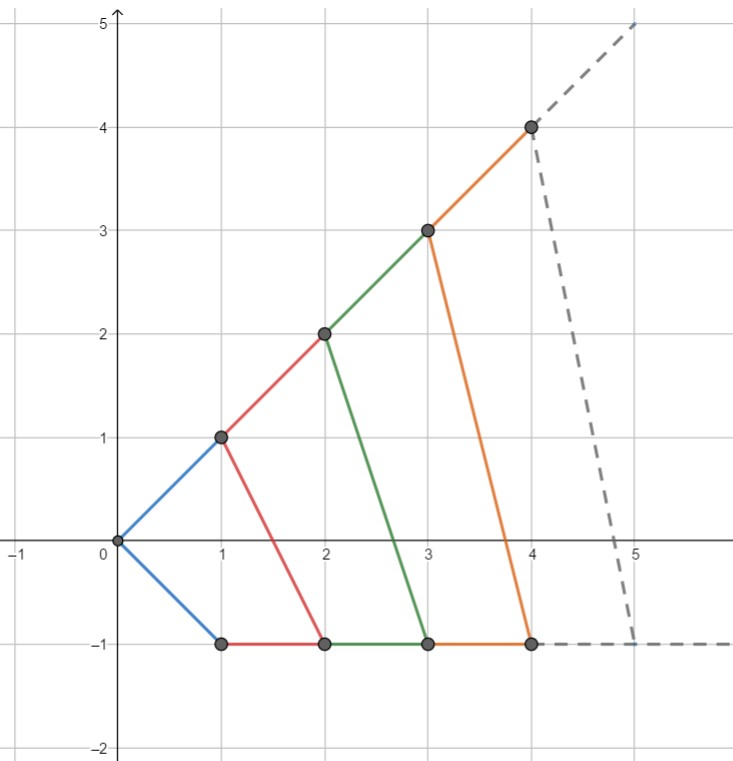
\includegraphics[scale=0.50]{martingalaex5.jpg}
  \end{figure}
\subsection*{ }
  \begin{enumerate}
  \item[(1)]
Osserviamo che per   n = 1 vale
  %\begin{align*}

  \[X_{1}=\begin{cases}-1 \,\,\, \text{se} \,\,\, \omega=1\\    +1 \,\,\, \text{se} \,\,\, \omega> 1\end{cases}\]
%  \[A_{-1}= \{\omega \in \Omega : \omega_1 = -1\} = 1;\]
%  \[A_{+1}= \{\omega \in \Omega : \omega_1 = +1\} = \omega \geq 2;\]
  \begin{equation*}
  \mathcal{F}_{1}=\sigma\{X_1\}=\sigma\{X_1^{-1}(A_{-1}), X_1^{-1}(A_{+1})\} = \sigma\{\{1\},[2, +\infty)\}.
  \end{equation*}
  %\{\{1\},[2, +\infty)\}.
% X_{1}\left(\omega\right)\in\{-1,1\},\\
% X_{2}\left(\omega\right)\in\{-1,2\},\\
%  ...\,\,\,\text{e così via}.
%  %\end{align*}
  Se ne deduce, allora, che, per $n > 0$
  \[X_{n}=\begin{cases}-1 \,\,\, \text{se} \,\,\, \omega\leq n\\    n \,\,\,\,\,\,\, \text{se} \,\,\, \omega> n\end{cases}\]
  e la filtrazione naturale del processo è: 
  \begin{equation*}
  \mathcal{F}_{n}=\sigma\{X_{0},...,X_{n}\}=\sigma\{\{1\},\{2\},...,\{n\}, [n+1
  , \infty)\}.
  \end{equation*}
  \item[(2)]
  Sia
  \begin{equation*}
  \mathbb{P}\left(A\right)=\sum_{k\in A}\frac{1}{k\left(k+1\right)}.
  \end{equation*}
  Mostriamo che $\mathbb{P}$ è una probabilità su $\left(\Omega,\mathcal{F}\right)$.
  \begin{itemize}
  \item[-]
  $\mathbb{P}\left(\emptyset\right)=0$, poiché, in tal caso, $\mathbb{P}\left(\emptyset\right)=\sum_{k\in \emptyset}\frac{1}{k\left(k+1\right)}$ è una sommatoria vuota, dato che non vi sono elementi in $\emptyset$;
  \item[-]
  $\mathbb{P}\left(A\right)\geq 0 \,\,\,\forall A\in \mathcal{F}$, poiché $\sum_{k\in A}\frac{1}{k\left(k+1\right)}> 0$ sempre, dato che $k \in \mathbb{N}\setminus\{0\}$;\\
  inoltre, se $A_{1},A_{2},...$ è una successione di insiemi mutuamente disgiunti in $\mathcal{F}$, allora 
  \item[-]
  $\mathbb{P}\left(\cup_{j=1}^{\infty}A_{j}\right)=\sum_{j=1}^{\infty}\mathbb{P}\left(A_{j}\right)$, poiché, in tal caso, è possibile scrivere
  \begin{align*}
  &\mathbb{P}\left(\cup_{j=1}^{\infty}A_{j}\right)=\sum_{k\in\cup_{j=1}^{\infty}A_{j}}\frac{1}{k\left(k+1\right)}=\sum_{k\in A_{1}}\frac{1}{k\left(k+1\right)}+\sum_{k\in A_{2}}\frac{1}{k\left(k+1\right)}+...=\\
  &\mathbb{P}\left(A_{1}\right)+\mathbb{P}\left(A_{2}\right)+...=\sum_{j=1}^{\infty}\mathbb{P}\left(A_{j}\right);
\end{align*}   
\item[-]
$\mathbb{P}\left(\Omega\right)=1$, poiché
\begin{equation*}
\mathbb{P}\left(\Omega\right)=\sum_{k=1}^{\infty}\frac{1}{k\left(k+1\right)}=\sum_{k=1}^{\infty}\left(\frac{1}{k}-\frac{1}{k+1}\right)
\end{equation*}
e, dunque,
\begin{align*}
&\sum_{n=1}^{k}\left(\frac{1}{n}-\frac{1}{n+1}\right)=\left(1-\frac{1}{2}\right)+\left(\frac{1}{2}-\frac{1}{3}\right)+...+\left(\frac{1}{k}-\frac{1}{k+1}\right)=\\
&1-\frac{1}{k+1}\longrightarrow 1, \,\,\, \text{per}\,\,\, k\rightarrow \infty.
\end{align*}
Infatti, ad esempio se n = 1 si ha:
\begin{align*}
&\mathbb{P}\left(X_1 = -1\right) = \frac{1}{k\left(k+1\right)}= \frac{1}{2}; \\
&\mathbb{P}\left(X_1 = +1\right) = \sum_{k=2}^{\infty}\frac{1}{k}-\frac{1}{k+1} = 1-\frac{1}{2} = \frac{1}{2};
\end{align*}
Per n = 2: 
\begin{align*}
&\mathbb{P}\left(X_1 = -1\right) =  \sum_{k=1}^{2}\frac{1}{k} - \frac{1}{k+1} = \frac{1}{2} + \frac{1}{6} = \frac{2}{3};\\
&\mathbb{P}\left(X_1 = +1\right) = \sum_{k=3}^{\infty}\frac{1}{k}-\frac{1}{k+1} = 1-\frac{2}{3} = \frac{1}{3};
\end{align*}
e così via. 
\end{itemize}
 
Mostriamo che $\left(X_{n}\right)_{n\geq 0}$ è una martingala rispetto a $\mathcal{F}_{n}$.
 \begin{itemize}
 \item
$\left(X_{n}\right)_{n\geq 0}$ è adattato a $\mathcal{F}_{n}$, poiché un processo stocastico è sempre adattato alla filtrazione naturale;
 \item
 $X_{n}\in L^{1}$, poiché
 \begin{align*}
  &\mathbb{E}[\mid X_{n}\mid]=\mid -1\mid\cdot\sum_{k= 1}^n \frac{1}{k(k+1)}+n\cdot\sum_{k=n+1}^{\infty} \frac{1}{k(k+1)} = 1 - \frac{1}{n+1} +\\
   &+n\cdot(1-(1-\frac{1}{n+1})) = 1 - \frac{1}{n+1} + \frac{n}{n+1} = \frac{2n}{n+1} < +\infty;
\end{align*}
\item
$\mathbb{E}[X_{n+1}\mid \mathcal{F}_{n}]= X_n$ poiché
\begin{align*}
\mathbb{E}[X_{n+1}\mid \mathcal{F}_{n}]=
&\mathbb{E}[X_{n+1}-X_{n} + X_{n}\mid \mathcal{F}_{n}]=\mathbb{E}[X_{n}\mid \mathcal{F}_{n}] +\mathbb{E}[X_{n+1}-X_{n}\mid \mathcal{F}_{n}]
\end{align*}
e, poiché $(X_{n+1} - X_n)$ è indipendente da $\mathbb{F}_{n}$ essendo ${X_n}$ un processo ad incrementi indipendenti e pertanto un processo di Markov, vale
\begin{align*}
&\mathbb{E}[X_{n+1}\mid \mathcal{F}_{n}]=
X_{n} + \mathbb{E}[X_{n+1} - X_{n}] =X_n+(-1)\cdot \sum_{k=1}^{n+1}\frac{1}{k} - \frac{1}{k+1} +\\
&+(n+1) \cdot \sum_{k=n+2}^{\infty}\frac{1}{k} - \frac{1}{k+1} - \left[(-1)\cdot\sum_{k=1}^{n}\frac{1}{k}-\frac{1}{k+1} + n \cdot \sum_{k=n+1}^{\infty}\frac{1}{k}-\frac{1}{k+1}\right]=\\
&X_n + (-1)\cdot\left(1-\frac{1}{n+2}\right)+(n+1)\left[1-\left(1-\frac{1}{n+2}\right)\right]+ \left(1-\frac{1}{n+1}\right)+\\
&-n\left[1-\left(1-\frac{1}{n+1}\right)\right]= X_n + \frac{n+2-(n+2)}{n+2}= X_n. 
 \end{align*}
 \end{itemize}
 \item[(3)]
La martingala $X_{n}$ è limitata in $L^{1}$, perché si ha che
 \begin{equation*}
\sup_{n} {\mathbb{E}[\lvert X_{n}\left(\omega\right)\lvert]}= \sup_{n} \frac{2n}{n+1} < \infty
 \end{equation*}
perciò applicando il teorema di convergenza di Doob si ottiene che 
 \begin{equation*}
 X_{n}\xrightarrow[]{q.c.}X_{\infty} \in L^{1}.
 \end{equation*}
  \end{enumerate}
  
   \newpage
  \section{}%---------------ESERCIZIO 6
  Sia $\Omega=\mathbb{N}\setminus \{0\}$, $\mathcal{F}=P\left(\Omega\right)$ e $\mathbb{P}\left(A\right)=\sum_{k\in A}2^{-k}$.\\
  Si consideri il seguente processo stocastico:
  \begin{equation*}
  \begin{cases} M_{n}=\omega \,\,\, \text{se} \,\,\, \omega\leq n\\M_{n}=n+2 \,\,\, \text{se} \,\,\, \omega> n\end{cases}.
  \end{equation*}
  \begin{figure}[htb]\centering
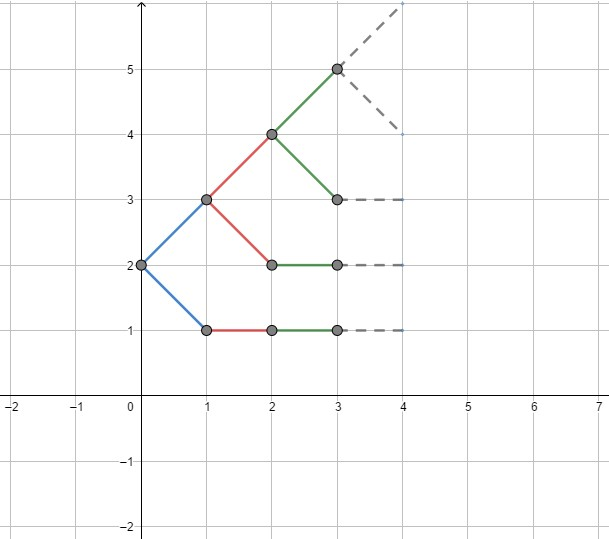
\includegraphics[scale=0.60]{martingalaex6.jpg}
  \end{figure}
  \begin{enumerate}
  \item[(1)]
  Mostriamo che $\mathbb{P}$ è una probabilità su $\left(\Omega,\mathcal{F}\right)$.
  \begin{itemize}
  \item[-]
  $\mathbb{P}\left(\emptyset\right)=0$, poiché, in tal caso, $\mathbb{P}\left(\emptyset\right)=\sum_{k\in \emptyset}\frac{1}{2^{k}}$ è una sommatoria vuota, dato che non vi sono elementi in $\emptyset$;
  \item[-]
  $\mathbb{P}\left(A\right)\geq 0 \,\,\,\forall A\in \mathcal{F}$, poiché $\frac{1}{2^{k}}> 0$ sempre;\\
  inoltre, se $A_{1},A_{2},...$ è una successione di insiemi mutuamente disgiunti in $\mathcal{F}$, allora 
  \item[-]
  $\mathbb{P}\left(\cup_{j=1}^{\infty}A_{j}\right)=\sum_{j=1}^{\infty}\mathbb{P}\left(A_{j}\right)$, poiché, in tal caso, è possibile scrivere
  \begin{align*}
\mathbb{P}\left(\cup_{j=1}^{\infty}A_{j}\right)=\sum_{k\in A_{1}}\frac{1}{2^{k}}+\sum_{k\in A_{2}}\frac{1}{2^{k}}+...=\mathbb{P}\left(A_{1}\right)+\mathbb{P}\left(A_{2}\right)+...=\sum_{j=1}^{\infty}\mathbb{P}\left(A_{j}\right);
\end{align*}   
\item[-]
$\mathbb{P}\left(\Omega\right)=1$ poiché, osservando che
\begin{equation*}
\sum_{n=1}^{\infty}2^{-n}=\sum_{n=0}^{\infty}\left(\frac{1}{2}\right)^{n}-1
\end{equation*}
in cui riconosciamo la serie geometrica di ragione $q= \frac{1}{2}$ e pertanto verifichiamo che
\begin{align*}
&\sum_{n=1}^{\infty}2^{-n}=\frac{1}{1-\frac{1}{2}} - 1= 2-1= 1.
\end{align*}
\end{itemize}


Mostriamo che $\left(M_{n}\right)_{n\geq 0}$ è una martingala rispetto alla filtrazione naturale \\$\mathcal{F}_{n}=\sigma\{M_{0},M_{1},...,M_{n}\}$.
 \begin{itemize}
 \item[-]
 $\left(M_{n}\right)_{n\geq 0}$ è adattato a $\mathcal{F}_{n}$, poiché un processo stocastico è sempre adattato alla filtrazione naturale;
 \item[-]
 $M_{n}\in L^{1}$, poiché
 \begin{align*}
  &\mathbb{E}[\lvert M_n \lvert] = \sum_{k=1}^{n} \frac{k}{2^k} + (n+2)\sum_{k=n+1}^{\infty} \frac{1}{2^k}=\\ 
&\frac{1}{\left(1-\frac{1}{2}\right)^2}\cdot \left[n\left(\frac{1}{2}\right)^{n+2}-(n+1)\left(\frac{1}{2}\right)^{n+1} +\frac{1}{2}\right]+(n+2)\left[\sum_{k=0}^{\infty} \frac{1}{2^k}-\sum_{k=0}^{n} \frac{1}{2^k}\right]=\\
 & =4n\left(\frac{1}{2}\right)^{n+2} -4(n+1)\left(\frac{1}{2}\right)^{n+1}+2+2(n+2)\left(\frac{1}{2}\right)^{n+1} = \\
 & =2 -2n\left(\frac{1}{2}\right)^{n+1}+4n\left(\frac{1}{2}\right)^{n+2}=2 < \infty; 
   \end{align*}
   \item[-]
   Con un ragionamento simile a quello dell'esercizio precedente possiamo far vedere facilmente che  
   \begin{align*}
&\mathbb{E}[M_{n+1} \lvert \mathcal{F}_n] = \mathbb{E}[M_{n+1}-M_{n}+M_{n} \lvert \mathcal{F}_{n}]= M_n + \mathbb{E}[M_{n+1} - M_n] =\\
&M_n+\sum_{k=0}^{n+1}\frac{k}{2^k}+(n+3)\sum_{k=n+2}^{\infty}\frac{1}{2^k}-\sum_{k=0}^{n}\frac{k}{2^k}-(n+2)\sum_{k=n+1}^{\infty}\frac{1}{2^k}=\\
&M_n + \frac{n+1}{2^{n+1}} + (n+2)\sum_{k=n+2}^\infty \frac{1}{2^k}-\left[(n+2)\sum_{k=n+2}^\infty \frac{1}{2^k}+\frac{n+2}{2^{n+1}}\right] + 1\cdot\sum_{k=n+2}^\infty \frac{1}{2^k} = \\
&M_n + \frac{n+1}{2^{n+1}} - \frac{n+2}{2^{n+1}} + \sum_{k=n+2}^\infty \frac{1}{2^k} = \frac{-1}{2^{n+1}}+2 - \frac{2^{n+2}-1}{2^{n+1}}-\frac{1}{2^{n+1}}=\\
&M_n -\frac{1}{2^{n+1}}+\frac{1}{2^{n+1}}=M_n.
   \end{align*}
   \end{itemize}  
   \newpage 
   \item[(2)]
   Per dimostrare che $M_n$ è una martingala ereditaria utilizziamo il teorema di caratterizzazione delle martingale in $L^1$. \\
Esso ci garantisce che se una martingala $M_n$ è uniformemente integrabile allora questa converge quasi certamente ed in $L^1$, e vale $M_n = \mathbb{E} \left[X \lvert \mathbb{F}_n \right]$ per qualche $X \in L^1$, cioè $M_n$ è una martingala ereditaria. \\Una famiglia di variabili aleatorie $X_i$ in uno spazio di probabilità $\left(\Omega, \mathcal{F}, \mathcal{F}_n, \mathcal{P}\right)$ è uniformemente integrabile se vale il limite 
   \[\lim_{M\rightarrow \infty} \left(\sup_i E(\lvert X_i\lvert; \lvert X_i\lvert > M)\right) = 0.\]
Si può scegliere un $M$ grande abbastanza tale che 
\[\sup_i \mathbb{E}\lvert X_i\lvert \leq M < \infty \]
ma, per quanto osservato in precedenza, $\mathbb{E}\lvert X_n \lvert$ non dipende da $n$ ma è un valore finito. Quindi si può concludere che $M_n$ è uniformemente integrabile e che pertanto è una martingala ereditaria per cui vale \[M_n = \mathbb{E}\left[X_\tau |\mathcal{F}_n\right] \] dove per $X_\tau$ si è scelta la martingala $M_n$ arrestata al tempo d'arresto finito $\tau$. \\
Dal teorema sovracitato, ma anche dal teorema di Doob e dal teorema di convergenza dominata si può inoltre affermare che la martingala $M_n$ converge non solo quasi certamente e in $L^p$, ma anche in $L^1$ al valore $M_\infty$, infatti si scrive
   \begin{equation*}
   M_{n}\xrightarrow[L^{1}]{q.c.}M_{\infty}\in L^{1},
   \end{equation*}
Infine, essendo $M_n$ ereditaria si può ancora affermare che vale \[  \lim_{n\to \infty} M_n = \lim_{n\to \infty} \mathbb{E}[X \lvert \mathcal{F}_n] =  \mathbb{E}[X\lvert\mathcal{F}_\infty]\]
cioè si può sempre supporla originata dal proprio limite e poiché $X_\tau$ é $\mathcal{F}_\infty$-misurabile allora si conclude che \[ \mathbb{E}[M_\infty\lvert\mathcal{F}_n] =  \mathbb{E}[X\lvert\mathcal{F}_n].\]
   
  \end{enumerate}
  
  
  \newpage
  \section{}%---------------ESERCIZIO 7
  \begin{enumerate}
  \item[(1)]
  Sia $M=\left(M_{n}\right)_{n\geq 0}$ una martingala ad incrementi equilimitati (cioè tale che $\mid M_{n}-M_{n-1}\mid\leq K$ con $K$ costante) e sia $M^{\tau}=\left(M_{n}^{\tau}\right)_{n\geq 0}$ la corrispondente martingala arrestata al tempo $\tau $, integrabile. Proviamo che $M^{\tau}$ è uniformemente integrabile.\\
  Sia
  \begin{equation*}
  M_{n}^{\tau}=M_{\tau\wedge 0}+\left(M_{\tau\wedge 1}-M_{\tau\wedge 0}\right)+\left(M_{\tau\wedge 2}-M_{\tau\wedge 1}\right)+....
  \end{equation*}
  Sfruttando l' ``identità di arresto''
  \begin{equation*}
  M_{n}^{\tau}-M_{n-1}^{\tau}=\left(M_{n}-M_{n-1}\right)\mathbbm{1}_{\tau\leq n},
  \end{equation*}
  otteniamo
  \begin{align*}
   M_{n}^{\tau}=M_{0}+\left(M_{1}-M_{0}\right)+\left(M_{2}-M_{1}\right)+...\\
   \Leftrightarrow\mid M_{n}^{\tau}\mid \leq \mid M_{0}\mid + \sum_{i=1}^{n}\mid M_{i}-M_{i-1}\mid \mathbbm{1}_{\{\tau\geq i\}}.
  \end{align*}
  Applicando la maggiorazione
  \begin{equation*}
\mid M_{n}^{\tau}\mid \leq \mid M_{0}\mid + \sum_{i=1}^{n}\mid M_{i}-M_{i-1}\mid \mathbbm{1}_{\{\tau\geq i\}}\leq \mid M_{0}\mid + \sum_{i=1}^{\infty}\mid M_{i}-M_{i-1}\mid \mathbbm{1}_{\{\tau\geq i\}},
     \end{equation*}
     ci basterà dimostrare che
     \begin{equation*}
     \mathbb{E}[\mid \sum_{i=1}^{\infty}\mid M_{i}-M_{i-1}\mid \mathbbm{1}_{\{\tau\geq i\}} \mid]<+\infty,
     \end{equation*}
     per poter dire che  $\mid M_{n}^{\tau}\mid\leq Z \in L^{1}$.\\
     In effetti, ciò è assicurato dal teorema di convergenza dominata di Beppo Levi, per il quale risulta che
     \begin{align*}
      &\mathbb{E}[\mid \sum_{i=1}^{\infty}\mid M_{i}-M_{i-1}\mid \mathbbm{1}_{\{\tau\geq i\}} \mid]\leq  \mathbb{E}[\sum_{i=1}^{\infty}K \mathbbm{1}_{\{\tau\geq i\}} ]=\\
      & \mathbb{E}[\lim\limits_{n\rightarrow \infty}\sum_{i=1}^{n}K\mathbbm{1}_{\{\tau\geq i\}}]=	\lim\limits_{n\rightarrow \infty}\mathbb{E}[\sum_{i=1}^{n}K\mathbbm{1}_{\{\tau\geq i\}}]=\\
      &\lim\limits_{n\rightarrow \infty}K\sum_{i=1}^{n}\mathbb{E}[\mathbbm{1}_{\{\tau\geq i\}}]=\lim\limits_{n\rightarrow \infty}K\sum_{i=1}^{n}P\left(\tau\geq i\right)=K\sum_{i=1}^{\infty}P\left(\tau\geq i\right)=K\mathbb{E}\left(\tau\right)<\infty
     \end{align*}
     (poiché $\tau$ è un tempo di arresto integrabile). \\
     Dunque,
     \begin{equation*}
     \mid M_{n}^{\tau}\mid \leq Z\in L^{1} \Rightarrow M_{n}^{\tau}\xrightarrow[L^{1}]{}M_{\tau}
     \end{equation*}
     ed essendo, quindi, $M_{n}^{\tau}$ limitata in $L^{1}$, per il ``teorema di convergenza'' di Doob, vale anche
     \begin{equation*}
     M_{n}^{\tau}\xrightarrow[]{q.c.}M_{\tau}\in L^{1}.
     \end{equation*}
     Allora, se
     \begin{equation*}
      M_{n}^{\tau}\xrightarrow[L^{1}]{q.c.}M_{\tau}\in L^{1},
     \end{equation*}
     per il ``teorema di caratterizzazione di martingale in $L^{1}$'', $M^{\tau}$ è uniformemente integrabile.
     \item[(2)]
     Sia $M=\left(M_{n}\right)_{n\geq 0}$ una martingala tale che:
     \begin{itemize}
     \item[i)]
     $M_{0}=0$;
     \item[ii)]
     $0<a\leq \mid M_{n}-M_{n-1}\mid \leq K <+\infty$.
     \end{itemize}
     \begin{figure}[htb]\centering
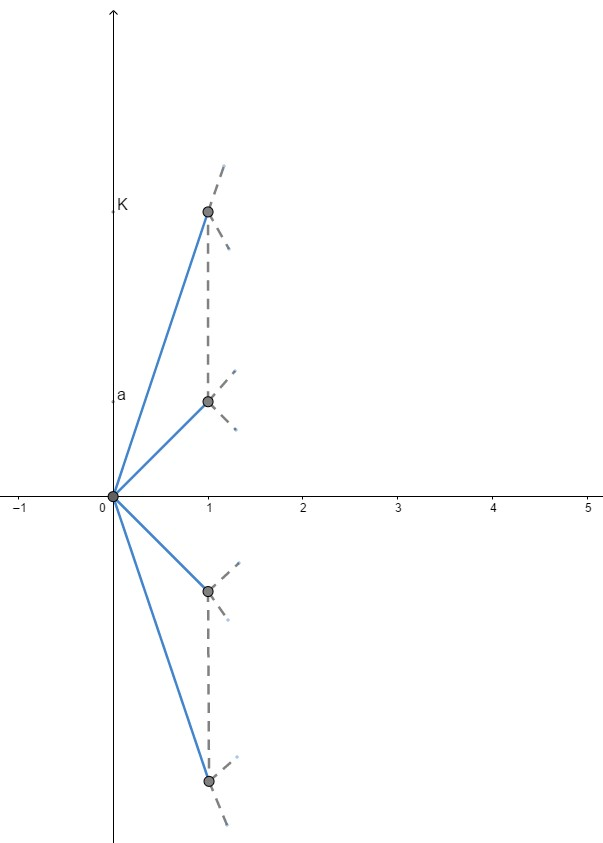
\includegraphics[scale=0.45]{martingalaex7.jpg}
  \end{figure}
  
  \newpage
  \begin{alphaparts}
  \questionpart
  La martingala in questione non converge q.c. al crescere di $n$. Questo perché essa, per $n\rightarrow \infty$, può espandersi simmetricamente verso valori infinitamente positivi e negativi.\\
  Se, per assurdo, $M_{n}$ convergesse q.c. a $M_{\infty}$, si avrebbe necessariamente che $M_{\infty}=0$, da cui
  \begin{equation*}
  \lim\limits_{n\rightarrow \infty}\mid M_{n}-M_{n-1}\mid=0 \,\lightning,
  \end{equation*}
   dal momento che $\mid M_{n}-M_{n-1}\mid\geq a>0$, $\forall n$. 
   \questionpart
   Sia $\lambda>0$ e sia $\tau=\inf{n:M_{n}>\lambda}$.\\
   Dal momento che $0<\lambda<\infty$, possiamo sicuramente affermare che $\tau$ è un tempo di arresto finito. Infatti, se la martingala $\left(M_{n}\right)_{n\geq 0}$, per $n\rightarrow +\infty$, si estende indefinitamente a $+\infty$ e $-\infty$,esisterà sicuramente un tempo di ingresso finito $\tau$, in cui essa assumerà il valore finito $\lambda + k$, per un opportuno valore $k\in \mathbb{R}$.\\
   Ne consegue che $\left(M_{n}^{\tau}\right)_{n\geq 0}$ è certamente una martingala.\\
   Proviamo che $\lambda+K-M_{n}^{\tau}$ è una martingala.
   \begin{itemize}
   \item[-]
   $\left(\lambda+K-M_{n}^{\tau}\right)\thicksim\mathcal{F}_{n}$, con $\mathcal{F}_{n}$ filtrazione naturale del processo $\left(\lambda+K-M_{n}^{\tau}\right)_{n\geq 0}$;
   \item[-]
   $\left(\lambda+K-M_{n}^{\tau}\right)\in L^{1}$, poiché $\left(\lambda+K\right)\in L^{1}$ e $M_{n}^{\tau}\in L^{1}$;
   \item[-]
   $\mathbb{E}[\lambda+K-M_{n+1}^{\tau}\mid \mathcal{F}_{n}]=\lambda+K-M_{n}^{\tau}$, poiché
   \begin{align*}
   \mathbb{E}[\lambda+K-M_{n+1}^{\tau}\mid \mathcal{F}_{n}]=\mathbb{E}[\lambda+K\mid \mathcal{F}_{n}]-\mathbb{E}[M_{n+1}^{\tau}\mid \mathcal{F}_{n}]=\lambda+K-M_{n}^{\tau}.
   \end{align*}
  \end{itemize}    
    Adesso, per provare che $\lambda+K-M_{n}^{\tau}$ è una martingala convergente, basta provare che $M_{n}^{\tau}$ è convergente.\\
    Usando l' ``identità di arresto'' e le proprietà del valore assoluto, si ottiene
    \begin{equation*}
    \mid M_{n}^{\tau}\mid \leq \sum_{i=1}^{n}\mid M_{i}-M_{i-1}\mid \mathbbm{1}_{\{\tau\geq i\}},
    \end{equation*}
    da cui:
    \begin{align*}
    &\mathbb{E}[\mid\sum_{i=1}^{n}\mid M_{i}-M_{i-1}\mid \mathbbm{1}_{\{\tau\geq i\}}\mid]\leq \mathbb{E}[\sum_{i=1}^{n}K\mathbbm{1}_{\{\tau\geq i\}}]=\\
    &K\sum_{i=1}^{n}\mathbb{E}[\mathbbm{1}_{\{\tau\geq i\}}]=K\sum_{i=1}^{n}P\left(\tau\geq i\right)<+\infty \\
 &\Rightarrow \sup_{n}{\mathbb{E}[\mid M_{n}^{\tau}\mid]}\leq +\infty.   
    \end{align*}
    Pertanto, per il ``teorema di convergenza'' di Doob,
    \begin{equation*}
    M_{n}^{\tau}\xrightarrow[]{q.c.} M_{\tau}\in L^{1}    
    \end{equation*}
    e, dunque, anche $\lambda +K-M_{n}^{\tau}$ converge q.c. a $\left(\lambda + K-M_{\tau}\right) \in L^{1}$.
    \questionpart
    Il ``teorema di arresto opzionale'' di Doob afferma che se $M=\left(M_{n}\right)_{n\geq 0}$ è una martingala su $\Omega$ e $\tau$ è un tempo di arresto per $M$, supponendo che valga una delle seguenti condizioni:
    \begin{itemize}
    \item[i)]
    $\tau$ è limitato, ovvero $\exists c$ costante tale che $\tau < c$ q.c.;
    \item[ii)]
    $\mathbb{E}[\tau]<\infty$ ed esiste una costante $K\in \mathbb{R}$ tale che
    \begin{align*}
    \mid M_{n}\left(\omega\right)-M_{n-1}\left(\omega\right)\mid \leq K \,\,\, \forall\left(n,\omega\right);
\end{align*}      
\item[iii)]
$M$ è limitata, ovvero $\exists K \in \mathbb{R}$ tale che
\begin{align*}
\mid M_{n}\left(\omega\right)\mid \leq K \,\,\, \forall\left(n,\omega\right)
\end{align*}
e $\tau$ è finito q.c.;
    \end{itemize}
    allora $\mathbb{E}[M_{\tau}]=\mathbb{E}[M_{0}]$.\\
    Nel caso della martingala $M=\left(M_{n}\right)_{n\geq 0}$, definita al punto (b), però, risulta che $\mathbb{E}[M_{0}]=0$, mentre $\lambda<\mathbb{E}[M_{\tau}]\leq \lambda + K$.\\
    Di conseguenza, $\mathbb{E}[M_{\tau}]\neq\mathbb{E}[M_{0}]$ e quindi, in particolare, $\tau$ non è integrabile. 
  \end{alphaparts}
  \end{enumerate}
  
% Sometimes questions get separated from their bodies. Use a \newpage to force
% them to wrap to the next page.
% Use \renewcommand{\questiontype}{<text>} to change what word is displayed
% before numbered questions
%\renewcommand{\questiontype}{Task}
\end{document}
